\documentclass[]{beamer}
\mode<presentation>
% Time-stamp: <2016-05-08 15:19:09 (jmiller)>

% beamer stuff
% Gives us the bottom line with all the goodies
\useoutertheme{infolines}
% Just the theme to use. Should be built into bemaer. Setting the
% height gets rid of a whole lot of whitespace
\usetheme[height=7mm]{Rochester}
\usefonttheme{serif}
% Usually beamer gives you navigation hyperlinks on the bottom
% right. I turned this off. It's annoying.
\setbeamertemplate{navigation symbols}{} 
% Makes my text boxes look pretty
\setbeamertemplate{blocks}[rounded][shadow=true] 
% Makes my bullet points 3d balls
\setbeamertemplate{items}[ball]

% Josh's packages
\usepackage{multimedia}
\usepackage{tabularx}
\usepackage{booktabs}
\usepackage{subfigure}
\usepackage{graphicx}
\usepackage{amsmath}
\usepackage{latexsym}
\usepackage{mathrsfs}

% Packages for me
\usepackage{amsmath,amssymb,latexsym}
\usepackage[mathscr]{eucal}
\usepackage{mathrsfs}
\usepackage{verbatim}
\usepackage{braket}
\usepackage{listings}
\usepackage{amsthm}
\usepackage{xcolor}
%\usepackage[usenames,dvipsnames,svgnames,table]{xcolor}
\usepackage{fancybox}
\usepackage{animate}
% \usepackage{media9}
\usepackage{multicol}
\usepackage{mdframed}
%\usepackage{scalerel}

% Macros

%Blackboard Bold
\newcommand{\R}{\mathbb{R}}
\newcommand{\Z}{\mathbb{Z}}
\newcommand{\N}{\mathbb{N}}
\newcommand{\Q}{\mathbb{Q}}
\newcommand{\A}{\mathbb{A}}
\newcommand{\E}{\mathbb{E}}
% other
\newcommand{\eval}{\biggr\rvert} %evaluated at
\newcommand{\myvec}[1]{\mathbf{#1}} % vectors for me
% total derivatives 
\newcommand{\diff}[2]{\frac{d #1}{d #2}} 
\newcommand{\dd}[1]{\frac{d}{d #1}}
% partial derivatives
\newcommand{\pd}[2]{\frac{\partial #1}{\partial #2}} 
\newcommand{\pdd}[1]{\frac{\partial}{\partial #1}} 
% Order operator
\DeclareRobustCommand{\orderof}{\ensuremath{\mathcal{O}}}

% tikz
\usepackage{tikz}
\usetikzlibrary{arrows}
\usepackage{pgfplots}

% define a really nice visible "purple"
\definecolor{gimppurple}{HTML}{AD26FB}
% a light grey
\definecolor{lightgrey}{HTML}{E0E0E0}

\newcommand{\backupbegin}{
   \newcounter{finalframe}
   \setcounter{finalframe}{\value{framenumber}}
}
\newcommand{\backupend}{
   \setcounter{framenumber}{\value{finalframe}}
}

\title[Comp. Phys.]{Solving Physics Problems on a Computer}
\author[J. Miller]{Jonah M. Miller}
\institute[PI]{\color{blue}Perimeter Institute for Theoretical Physics}

\date[Lunch \& Learn]{\color{black}Lunch and Learn\\May 5, 2016}

\begin{document}

\begin{frame}[plain]
\titlepage
\end{frame}

\begin{frame}{Agenda (time permitting)}
\tableofcontents
\end{frame}

\section{Throwing Darts for $\pi$}
\label{sec:darts}

\begin{frame}
  \frametitle{The Random Darts Player}
  \begin{columns}
    \column{6cm}
    \begin{center}
      \animategraphics[width=6cm,every1,autoplay,loop]{1}{figures/darts-frame-}{0}{5}
    \end{center}
    \column{6cm}
    \begin{center}
      \includegraphics[width=6cm]{figures/Darts_gameplay}
    \end{center}
  \end{columns}
\end{frame}

\begin{frame}
  \frametitle{The Darts Tell us the Area of the Ring!}
  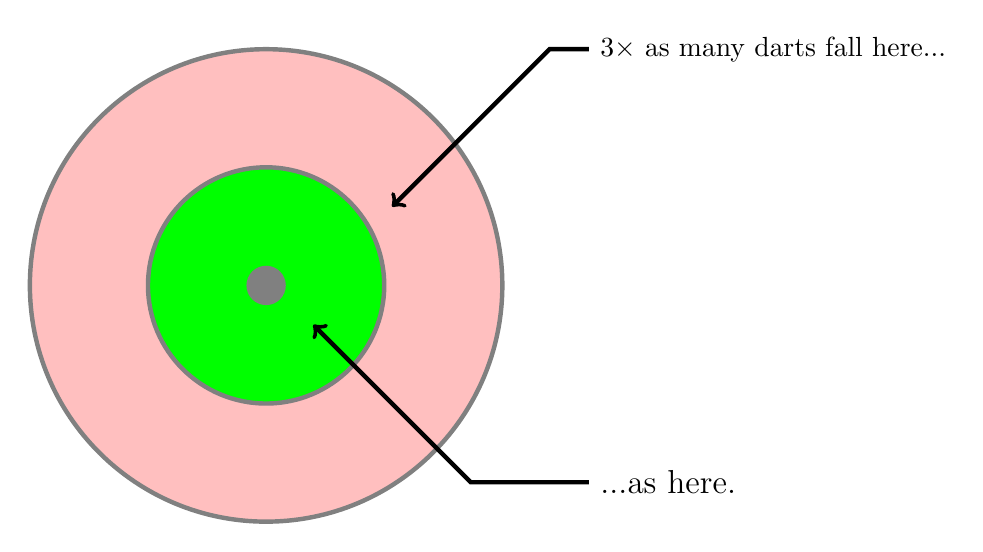
\begin{tikzpicture}
      \coordinate (bcenter) at (3.4cm,4cm);
      \fill[color=pink] (bcenter) circle(3cm);
      \fill[color=green] (bcenter) circle (1.5cm);
      \draw[color=gray,ultra thick] (bcenter) circle (1.5cm);
      \draw[color=gray,ultra thick] (bcenter) circle (3cm);
      \fill[color=gray] (bcenter) circle (0.25cm);
      \draw[color=black,ultra thick,<-] 
      (5cm,5cm) --(7cm,7cm) 
      -- (7.5cm,7cm)
      node[right] {$3\times$ as many darts fall here...};
      \draw[color=black,ultra thick,<-]
      (4cm,3.5cm) -- (6cm,1.5cm) 
      -- (7.5cm,1.5cm) 
      node[right] {\large...as here.};
    \end{tikzpicture}
\end{frame}

\begin{frame}
  \frametitle{Darts and $\pi$}
  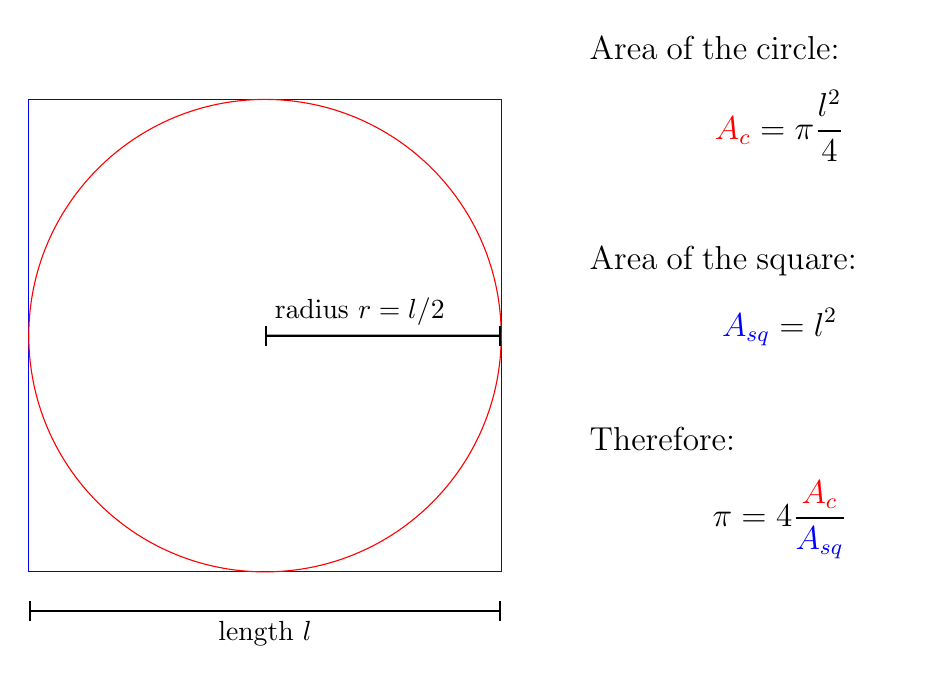
\begin{tikzpicture}
    \coordinate(bcenter) at (4cm,4cm);
    \draw[color=blue] (1,1) rectangle (7,7);
    \draw[color=red] (bcenter) circle (3cm);
    \draw[thick,|-|] (1,0.5) -- (7,0.5);
    \draw (4,0.5) node[below] {length $l$};
    \draw[thick,|-|] (bcenter) -- (7,4);
    \draw (4cm,4.3cm) node[right] {radius $r = l/2$};
    \draw (8,7) node[right,text width=4cm] 
    {\large Area of the circle:
      $$\qquad {\color{red}A_{c}} = \pi \frac{l^2}{4}$$};
    \draw (8,4.5) node[right,text width=4cm]
    {\large Area of the square:
      $$\qquad {\color{blue}A_{sq}} = l^2$$};
    \draw (8,2) node[right,text width=4cm]
    {\large Therefore:
      $$\qquad \pi = 4\frac{\color{red}A_c}{\color{blue}A_{sq}}$$};
  \end{tikzpicture}
\end{frame}

\section{Planetary Orbits a la Newton}
\label{sec:newton}

\begin{frame}
  \frametitle{Newton's Laws}
\end{frame}

\section{Structure of a Star}
\label{sec:star}

\begin{frame}
  \frametitle{Math is our X-Ray Vision}
\end{frame}

\end{document}